\section{Ergonomische Inspektion}

Eine der relevanten Aufgaben, die zu Beginn der Analyse einer Schnittstelle durchgeführt werden muss, ist eine ergonomische Inspektion der Schnittstelle.
Diese Aufgabe erfordert nur das Wissen, das für diese Bewertung erforderlich ist, keine Drittparteien oder externen Benutzer.

Für diese Inspektion werde ich mich hauptsächlich auf die ergonomischen Kriterien stützen, die von J. M. C. Bastien und D. L. Scapin in ihrem Artikel \textit{Ergonomic Criteria for the Evaluation of Human-Computer Interfaces}\cite{bastienscapin}.
Diese Kriterien, die in acht Punkte unterteilt sind, wurden entwickelt, um die Dimensionen der Funktionalität einer Schnittstelle zu definieren und zu operationalisieren.

Sie können folgendermaßen zusammengefasst werden:

\begin{table}[H]
  \begin{tabular}{p{0.25\linewidth} |p{0.5\linewidth}|p{0.25\linewidth}}
    Name                  & Beschreibung                                                                                                                                                                                 & Unterkriterien                                                            \\ \hline\hline

    Guidance              & Mittel, die zur Verfügung stehen, um die Benutzer während ihrer Interaktion mit einem Computer zu beraten, zu orientieren, zu informieren, anzuweisen und zu leiten                          & Prompting, Grouping/Distinction of Items, Immediate Feedback, Legibility. \\\hline
    Workload              & betrifft alle Schnittstellenelemente, die eine Rolle bei der Verringerung der wahrnehmungsbedingten oder kognitiven Belastung der Nutzer und bei der Steigerung der Dialogeffizienz spielen. & Brevity, Information Density                                              \\\hline
    Explicit Control      & Verarbeitung expliziter Benutzeraktionen durch das System und die Kontrolle, die die Benutzer über die Verarbeitung ihrer Aktionen durch das System ausüben.                                 & Explicit User Action,  User Control                                       \\\hline
    Adaptability          & Fähigkeit, sich kontextabhängig und entsprechend den Bedürfnissen und Vorlieben der Nutzer zu verhalten                                                                                      & Flexibility, User Experience                                              \\\hline
    Error Management      & Vorbeugung und Reduzierung von Fehlern und Behebung von Fehlern, wenn sie auftreten                                                                                                          & Error Protection, Quality of Error Messages, Error Correction             \\\hline
    Consistency           & die Art und Weise, in der Entscheidungen für das Schnittstellendesign in ähnlichen Kontexten beibehalten werden und in unterschiedlichen Kontexten anders ausfallen                          &                                                                           \\\hline
    Significance of Codes & Beziehung zwischen einem Begriff und/oder einem Zeichen und seiner Referenz.                                                                                                                 &                                                                           \\\hline
    Compatibility         & Übereinstimmung zwischen den Merkmalen der Benutzer und den Merkmalen der Aufgabe sowie die Organisation der Ausgaben, Eingaben und des Dialogs für eine bestimmte Anwendung,                &
  \end{tabular}
  \caption{Zusammenfassung der ergonomischen Kriterien von Bastien und Scapin}
\end{table}

Die Inspektion wurde über einen Zeitraum von zwei Wochen durchgeführt. Die Methodik bestand darin, für jedes Kriterium alle Seiten der Benutzeroberfläche durchzugehen und Mängel zu identifizieren.
Dies führte zu einem Inspektionsbericht (pdf-Version in Englisch \ref{dryad-ergonomic-inspection}), in dem jedes Problem detailliert und mit einem Lösungsansatz beschrieben wurde. Angesichts der umfassenden Liste mussten die Aufgaben priorisiert werden.
Dies geschah in Absprache mit dem Cloud-Team.
Die kritischsten Punkte werden in den folgenden Abschnitten nach Kriterien gegliedert.

\subsection{Guidance}

Ein häufig anzutreffender Mangel in Schnittstellen ist das Fehlen von Labels in den Eingaben eines Formulars oder das Verwenden nur eines Icons.
Dies passt zum Unterkriterium \textit{Prompting} und stellt ein echtes Verständnisrisiko für den Nutzer dar.
Obwohl viele Icons von der Mehrheit der Menschen als üblich angesehen werden, bleibt es ein Risiko, sie zu verwenden, vor allem, wenn die Schnittstelle für mehrere Kulturtypen oder mehrere Ebenen der Computerkenntnisse auf Seiten der Benutzer bestimmt ist.
Preethy PAPPACHAN und Martina ZIEFLE haben in ihrer Studie \textit{Cultural Influences on the Comprehensibility of Icons in Mobile-Computer-Interaction}\cite{iconsCultureInfluence} nachgewiesen, dass Icons in allen Kulturen im Allgemeinen als das erkannt werden, was sie darstellen, aber nicht als das, was sie bedeuten, was jedoch für die Verständlichkeit von Icons von großer Bedeutung ist.
So ist es notwendig, dass die Benutzeroberfläche Daten mit einer Erklärung präsentiert, die nicht nur ikonografisch ist, wie es auf dem folgenden Screenshot leider der Fall ist.

\begin{figure}[H]
  \centering
  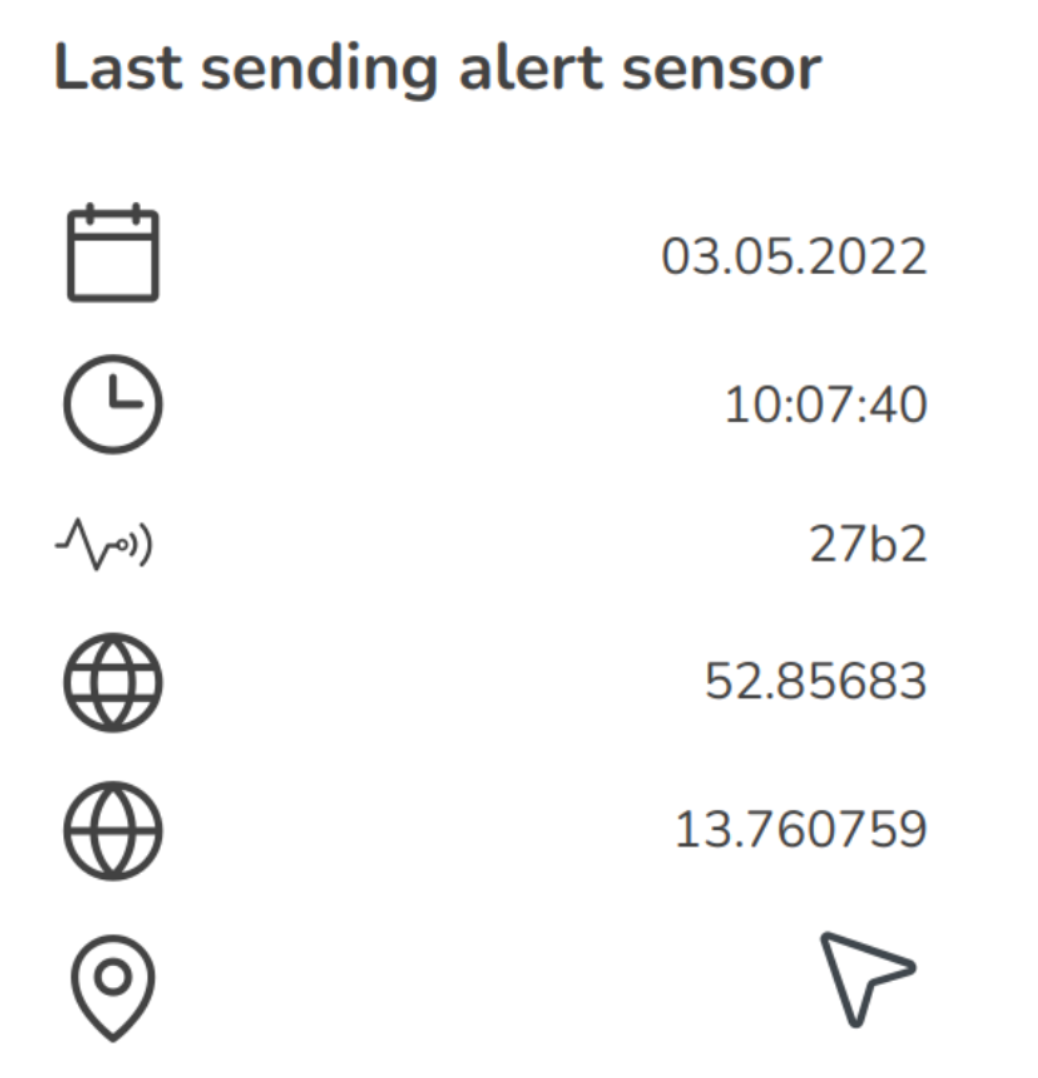
\includegraphics[width=4cm]{app_label_icon}
  \caption{Darstellung mit Icons als einzigem Label.}
\end{figure}

% [TODO]: add solution?
